\section{Como incluir gráficos em R no artigo.}

Inclua gráficos explicativos com R. Seguem alguns exemplos:

\begin{figure}
    \centering
    % Created by tikzDevice version 0.12.3.1 on 2022-05-25 11:36:55
% !TEX encoding = UTF-8 Unicode
\begin{tikzpicture}[x=1pt,y=1pt]
\definecolor{fillColor}{RGB}{255,255,255}
\path[use as bounding box,fill=fillColor,fill opacity=0.00] (0,0) rectangle (308.44,270.16);
\begin{scope}
\path[clip] ( 49.20, 61.20) rectangle (283.24,220.96);
\definecolor{drawColor}{RGB}{0,0,255}

\path[draw=drawColor,line width= 0.4pt,line join=round,line cap=round] ( 57.87, 79.44) --
	(112.04,104.10) --
	(166.22,141.08) --
	(220.40,116.42) --
	(274.57,178.06);

\path[draw=drawColor,line width= 0.4pt,line join=round,line cap=round] ( 57.87, 79.44) circle (  2.25);

\path[draw=drawColor,line width= 0.4pt,line join=round,line cap=round] (112.04,104.10) circle (  2.25);

\path[draw=drawColor,line width= 0.4pt,line join=round,line cap=round] (166.22,141.08) circle (  2.25);

\path[draw=drawColor,line width= 0.4pt,line join=round,line cap=round] (220.40,116.42) circle (  2.25);

\path[draw=drawColor,line width= 0.4pt,line join=round,line cap=round] (274.57,178.06) circle (  2.25);
\end{scope}
\begin{scope}
\path[clip] (  0.00,  0.00) rectangle (308.44,270.16);
\definecolor{drawColor}{RGB}{0,0,0}

\path[draw=drawColor,line width= 0.4pt,line join=round,line cap=round] ( 57.87, 61.20) -- (274.57, 61.20);

\path[draw=drawColor,line width= 0.4pt,line join=round,line cap=round] ( 57.87, 61.20) -- ( 57.87, 55.20);

\path[draw=drawColor,line width= 0.4pt,line join=round,line cap=round] (112.04, 61.20) -- (112.04, 55.20);

\path[draw=drawColor,line width= 0.4pt,line join=round,line cap=round] (166.22, 61.20) -- (166.22, 55.20);

\path[draw=drawColor,line width= 0.4pt,line join=round,line cap=round] (220.40, 61.20) -- (220.40, 55.20);

\path[draw=drawColor,line width= 0.4pt,line join=round,line cap=round] (274.57, 61.20) -- (274.57, 55.20);

\node[text=drawColor,anchor=base,inner sep=0pt, outer sep=0pt, scale=  1.00] at ( 57.87, 39.60) {Mon};

\node[text=drawColor,anchor=base,inner sep=0pt, outer sep=0pt, scale=  1.00] at (112.04, 39.60) {Tue};

\node[text=drawColor,anchor=base,inner sep=0pt, outer sep=0pt, scale=  1.00] at (166.22, 39.60) {Wed};

\node[text=drawColor,anchor=base,inner sep=0pt, outer sep=0pt, scale=  1.00] at (220.40, 39.60) {Thu};

\node[text=drawColor,anchor=base,inner sep=0pt, outer sep=0pt, scale=  1.00] at (274.57, 39.60) {Fri};

\path[draw=drawColor,line width= 0.4pt,line join=round,line cap=round] ( 49.20, 67.12) -- ( 49.20,220.96);

\path[draw=drawColor,line width= 0.4pt,line join=round,line cap=round] ( 49.20, 67.12) -- ( 43.20, 67.12);

\path[draw=drawColor,line width= 0.4pt,line join=round,line cap=round] ( 49.20,116.42) -- ( 43.20,116.42);

\path[draw=drawColor,line width= 0.4pt,line join=round,line cap=round] ( 49.20,165.73) -- ( 43.20,165.73);

\path[draw=drawColor,line width= 0.4pt,line join=round,line cap=round] ( 49.20,215.04) -- ( 43.20,215.04);

\node[text=drawColor,anchor=base east,inner sep=0pt, outer sep=0pt, scale=  1.00] at ( 37.20, 63.67) {0};

\node[text=drawColor,anchor=base east,inner sep=0pt, outer sep=0pt, scale=  1.00] at ( 37.20,112.98) {4};

\node[text=drawColor,anchor=base east,inner sep=0pt, outer sep=0pt, scale=  1.00] at ( 37.20,162.29) {8};

\node[text=drawColor,anchor=base east,inner sep=0pt, outer sep=0pt, scale=  1.00] at ( 37.20,211.60) {12};

\path[draw=drawColor,line width= 0.4pt,line join=round,line cap=round] ( 49.20, 61.20) --
	(283.24, 61.20) --
	(283.24,220.96) --
	( 49.20,220.96) --
	( 49.20, 61.20);
\end{scope}
\begin{scope}
\path[clip] ( 49.20, 61.20) rectangle (283.24,220.96);
\definecolor{drawColor}{RGB}{255,0,0}

\path[draw=drawColor,line width= 0.4pt,dash pattern=on 4pt off 4pt ,line join=round,line cap=round] ( 57.87, 91.77) --
	(112.04,128.75) --
	(166.22,116.42) --
	(220.40,128.75) --
	(274.57,215.04);

\path[draw=drawColor,line width= 0.4pt,line join=round,line cap=round] ( 55.87, 89.78) rectangle ( 59.86, 93.76);

\path[draw=drawColor,line width= 0.4pt,line join=round,line cap=round] (110.05,126.76) rectangle (114.04,130.75);

\path[draw=drawColor,line width= 0.4pt,line join=round,line cap=round] (164.23,114.43) rectangle (168.22,118.42);

\path[draw=drawColor,line width= 0.4pt,line join=round,line cap=round] (218.40,126.76) rectangle (222.39,130.75);

\path[draw=drawColor,line width= 0.4pt,line join=round,line cap=round] (272.58,213.05) rectangle (276.57,217.03);
\end{scope}
\begin{scope}
\path[clip] (  0.00,  0.00) rectangle (308.44,270.16);
\definecolor{drawColor}{RGB}{0,128,0}

\node[text=drawColor,anchor=base,inner sep=0pt, outer sep=0pt, scale=  1.00] at (166.22, 15.60) {Days};

\node[text=drawColor,rotate= 90.00,anchor=base,inner sep=0pt, outer sep=0pt, scale=  1.00] at ( 10.80,141.08) {Total};
\end{scope}
\begin{scope}
\path[clip] ( 49.20, 61.20) rectangle (283.24,220.96);
\definecolor{drawColor}{RGB}{0,0,255}

\path[draw=drawColor,line width= 0.8pt,line join=round,line cap=round] ( 60.03,205.44) -- ( 74.43,205.44);
\definecolor{drawColor}{RGB}{255,0,0}

\path[draw=drawColor,line width= 0.8pt,dash pattern=on 4pt off 4pt ,line join=round,line cap=round] ( 60.03,195.84) -- ( 74.43,195.84);
\definecolor{drawColor}{RGB}{0,0,255}

\path[draw=drawColor,line width= 0.8pt,line join=round,line cap=round] ( 67.23,205.44) circle (  1.80);
\definecolor{drawColor}{RGB}{255,0,0}

\path[draw=drawColor,line width= 0.8pt,line join=round,line cap=round] ( 65.63,194.24) rectangle ( 68.82,197.43);
\definecolor{drawColor}{RGB}{0,0,0}

\node[text=drawColor,anchor=base west,inner sep=0pt, outer sep=0pt, scale=  0.80] at ( 81.63,202.68) {cars};

\node[text=drawColor,anchor=base west,inner sep=0pt, outer sep=0pt, scale=  0.80] at ( 81.63,193.08) {trucks};
\end{scope}
\end{tikzpicture}

    \caption{Gráfico de linha.}
    \label{graph:linha}
\end{figure}

\FloatBarrier % Força a imagem a ser inserida entre o texto


Posso fazer uma citação ao gráfico também (Fig.~\ref{graph:linha}).

\begin{figure}
    %TODO: Ajustar tamanho
    \centering
    % Created by tikzDevice version 0.12.3.1 on 2022-05-25 11:52:22
% !TEX encoding = UTF-8 Unicode
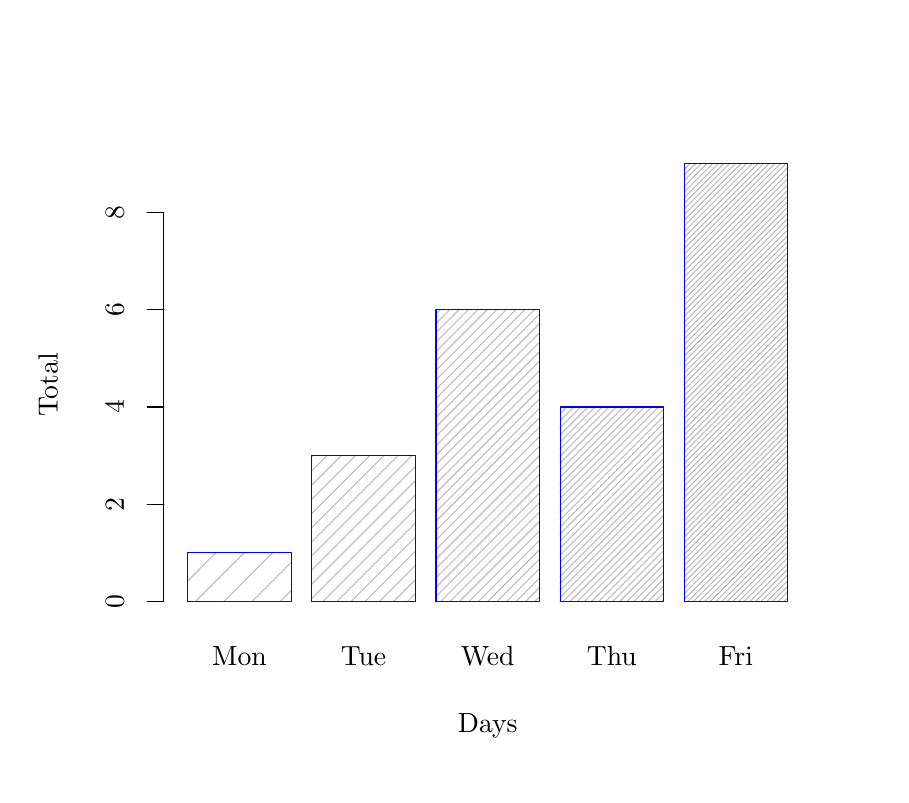
\begin{tikzpicture}[x=1pt,y=1pt]
\definecolor{fillColor}{RGB}{255,255,255}
\path[use as bounding box,fill=fillColor,fill opacity=0.00] (0,0) rectangle (308.44,270.16);
\begin{scope}
\path[clip] (  0.00,  0.00) rectangle (308.44,270.16);
\definecolor{drawColor}{RGB}{190,190,190}

\path[draw=drawColor,line width= 0.4pt,line join=round,line cap=round] ( 57.87, 70.25) -- ( 67.97, 80.36);

\path[draw=drawColor,line width= 0.4pt,line join=round,line cap=round] ( 60.62, 62.78) -- ( 78.19, 80.36);

\path[draw=drawColor,line width= 0.4pt,line join=round,line cap=round] ( 70.84, 62.78) -- ( 88.41, 80.36);

\path[draw=drawColor,line width= 0.4pt,line join=round,line cap=round] ( 81.06, 62.78) -- ( 95.23, 76.96);

\path[draw=drawColor,line width= 0.4pt,line join=round,line cap=round] ( 91.28, 62.78) -- ( 95.23, 66.74);

\path[draw=drawColor,line width= 0.4pt,line join=round,line cap=round] (102.70,115.09) -- (103.12,115.51);

\path[draw=drawColor,line width= 0.4pt,line join=round,line cap=round] (102.70,109.98) -- (108.23,115.51);

\path[draw=drawColor,line width= 0.4pt,line join=round,line cap=round] (102.70,104.87) -- (113.34,115.51);

\path[draw=drawColor,line width= 0.4pt,line join=round,line cap=round] (102.70, 99.76) -- (118.45,115.51);

\path[draw=drawColor,line width= 0.4pt,line join=round,line cap=round] (102.70, 94.65) -- (123.56,115.51);

\path[draw=drawColor,line width= 0.4pt,line join=round,line cap=round] (102.70, 89.54) -- (128.67,115.51);

\path[draw=drawColor,line width= 0.4pt,line join=round,line cap=round] (102.70, 84.43) -- (133.78,115.51);

\path[draw=drawColor,line width= 0.4pt,line join=round,line cap=round] (102.70, 79.32) -- (138.89,115.51);

\path[draw=drawColor,line width= 0.4pt,line join=round,line cap=round] (102.70, 74.21) -- (140.07,111.57);

\path[draw=drawColor,line width= 0.4pt,line join=round,line cap=round] (102.70, 69.10) -- (140.07,106.46);

\path[draw=drawColor,line width= 0.4pt,line join=round,line cap=round] (102.70, 63.99) -- (140.07,101.35);

\path[draw=drawColor,line width= 0.4pt,line join=round,line cap=round] (106.61, 62.78) -- (140.07, 96.24);

\path[draw=drawColor,line width= 0.4pt,line join=round,line cap=round] (111.72, 62.78) -- (140.07, 91.13);

\path[draw=drawColor,line width= 0.4pt,line join=round,line cap=round] (116.83, 62.78) -- (140.07, 86.02);

\path[draw=drawColor,line width= 0.4pt,line join=round,line cap=round] (121.94, 62.78) -- (140.07, 80.91);

\path[draw=drawColor,line width= 0.4pt,line join=round,line cap=round] (127.05, 62.78) -- (140.07, 75.80);

\path[draw=drawColor,line width= 0.4pt,line join=round,line cap=round] (132.16, 62.78) -- (140.07, 70.69);

\path[draw=drawColor,line width= 0.4pt,line join=round,line cap=round] (137.27, 62.78) -- (140.07, 65.58);

\path[draw=drawColor,line width= 0.4pt,line join=round,line cap=round] (147.54,166.74) -- (149.03,168.23);

\path[draw=drawColor,line width= 0.4pt,line join=round,line cap=round] (147.54,163.33) -- (152.44,168.23);

\path[draw=drawColor,line width= 0.4pt,line join=round,line cap=round] (147.54,159.93) -- (155.85,168.23);

\path[draw=drawColor,line width= 0.4pt,line join=round,line cap=round] (147.54,156.52) -- (159.25,168.23);

\path[draw=drawColor,line width= 0.4pt,line join=round,line cap=round] (147.54,153.11) -- (162.66,168.23);

\path[draw=drawColor,line width= 0.4pt,line join=round,line cap=round] (147.54,149.71) -- (166.07,168.23);

\path[draw=drawColor,line width= 0.4pt,line join=round,line cap=round] (147.54,146.30) -- (169.47,168.23);

\path[draw=drawColor,line width= 0.4pt,line join=round,line cap=round] (147.54,142.89) -- (172.88,168.23);

\path[draw=drawColor,line width= 0.4pt,line join=round,line cap=round] (147.54,139.48) -- (176.29,168.23);

\path[draw=drawColor,line width= 0.4pt,line join=round,line cap=round] (147.54,136.08) -- (179.69,168.23);

\path[draw=drawColor,line width= 0.4pt,line join=round,line cap=round] (147.54,132.67) -- (183.10,168.23);

\path[draw=drawColor,line width= 0.4pt,line join=round,line cap=round] (147.54,129.26) -- (184.90,166.63);

\path[draw=drawColor,line width= 0.4pt,line join=round,line cap=round] (147.54,125.86) -- (184.90,163.22);

\path[draw=drawColor,line width= 0.4pt,line join=round,line cap=round] (147.54,122.45) -- (184.90,159.81);

\path[draw=drawColor,line width= 0.4pt,line join=round,line cap=round] (147.54,119.04) -- (184.90,156.41);

\path[draw=drawColor,line width= 0.4pt,line join=round,line cap=round] (147.54,115.64) -- (184.90,153.00);

\path[draw=drawColor,line width= 0.4pt,line join=round,line cap=round] (147.54,112.23) -- (184.90,149.59);

\path[draw=drawColor,line width= 0.4pt,line join=round,line cap=round] (147.54,108.82) -- (184.90,146.19);

\path[draw=drawColor,line width= 0.4pt,line join=round,line cap=round] (147.54,105.42) -- (184.90,142.78);

\path[draw=drawColor,line width= 0.4pt,line join=round,line cap=round] (147.54,102.01) -- (184.90,139.37);

\path[draw=drawColor,line width= 0.4pt,line join=round,line cap=round] (147.54, 98.60) -- (184.90,135.97);

\path[draw=drawColor,line width= 0.4pt,line join=round,line cap=round] (147.54, 95.20) -- (184.90,132.56);

\path[draw=drawColor,line width= 0.4pt,line join=round,line cap=round] (147.54, 91.79) -- (184.90,129.15);

\path[draw=drawColor,line width= 0.4pt,line join=round,line cap=round] (147.54, 88.38) -- (184.90,125.75);

\path[draw=drawColor,line width= 0.4pt,line join=round,line cap=round] (147.54, 84.98) -- (184.90,122.34);

\path[draw=drawColor,line width= 0.4pt,line join=round,line cap=round] (147.54, 81.57) -- (184.90,118.93);

\path[draw=drawColor,line width= 0.4pt,line join=round,line cap=round] (147.54, 78.16) -- (184.90,115.52);

\path[draw=drawColor,line width= 0.4pt,line join=round,line cap=round] (147.54, 74.75) -- (184.90,112.12);

\path[draw=drawColor,line width= 0.4pt,line join=round,line cap=round] (147.54, 71.35) -- (184.90,108.71);

\path[draw=drawColor,line width= 0.4pt,line join=round,line cap=round] (147.54, 67.94) -- (184.90,105.30);

\path[draw=drawColor,line width= 0.4pt,line join=round,line cap=round] (147.54, 64.53) -- (184.90,101.90);

\path[draw=drawColor,line width= 0.4pt,line join=round,line cap=round] (149.19, 62.78) -- (184.90, 98.49);

\path[draw=drawColor,line width= 0.4pt,line join=round,line cap=round] (152.60, 62.78) -- (184.90, 95.08);

\path[draw=drawColor,line width= 0.4pt,line join=round,line cap=round] (156.01, 62.78) -- (184.90, 91.68);

\path[draw=drawColor,line width= 0.4pt,line join=round,line cap=round] (159.41, 62.78) -- (184.90, 88.27);

\path[draw=drawColor,line width= 0.4pt,line join=round,line cap=round] (162.82, 62.78) -- (184.90, 84.86);

\path[draw=drawColor,line width= 0.4pt,line join=round,line cap=round] (166.23, 62.78) -- (184.90, 81.46);

\path[draw=drawColor,line width= 0.4pt,line join=round,line cap=round] (169.64, 62.78) -- (184.90, 78.05);

\path[draw=drawColor,line width= 0.4pt,line join=round,line cap=round] (173.04, 62.78) -- (184.90, 74.64);

\path[draw=drawColor,line width= 0.4pt,line join=round,line cap=round] (176.45, 62.78) -- (184.90, 71.24);

\path[draw=drawColor,line width= 0.4pt,line join=round,line cap=round] (179.86, 62.78) -- (184.90, 67.83);

\path[draw=drawColor,line width= 0.4pt,line join=round,line cap=round] (183.26, 62.78) -- (184.90, 64.42);

\path[draw=drawColor,line width= 0.4pt,line join=round,line cap=round] (192.38,130.66) -- (194.79,133.08);

\path[draw=drawColor,line width= 0.4pt,line join=round,line cap=round] (192.38,128.11) -- (197.35,133.08);

\path[draw=drawColor,line width= 0.4pt,line join=round,line cap=round] (192.38,125.55) -- (199.90,133.08);

\path[draw=drawColor,line width= 0.4pt,line join=round,line cap=round] (192.38,123.00) -- (202.46,133.08);

\path[draw=drawColor,line width= 0.4pt,line join=round,line cap=round] (192.38,120.44) -- (205.01,133.08);

\path[draw=drawColor,line width= 0.4pt,line join=round,line cap=round] (192.38,117.89) -- (207.57,133.08);

\path[draw=drawColor,line width= 0.4pt,line join=round,line cap=round] (192.38,115.33) -- (210.12,133.08);

\path[draw=drawColor,line width= 0.4pt,line join=round,line cap=round] (192.38,112.78) -- (212.68,133.08);

\path[draw=drawColor,line width= 0.4pt,line join=round,line cap=round] (192.38,110.22) -- (215.24,133.08);

\path[draw=drawColor,line width= 0.4pt,line join=round,line cap=round] (192.38,107.67) -- (217.79,133.08);

\path[draw=drawColor,line width= 0.4pt,line join=round,line cap=round] (192.38,105.11) -- (220.35,133.08);

\path[draw=drawColor,line width= 0.4pt,line join=round,line cap=round] (192.38,102.56) -- (222.90,133.08);

\path[draw=drawColor,line width= 0.4pt,line join=round,line cap=round] (192.38,100.00) -- (225.46,133.08);

\path[draw=drawColor,line width= 0.4pt,line join=round,line cap=round] (192.38, 97.45) -- (228.01,133.08);

\path[draw=drawColor,line width= 0.4pt,line join=round,line cap=round] (192.38, 94.89) -- (229.74,132.25);

\path[draw=drawColor,line width= 0.4pt,line join=round,line cap=round] (192.38, 92.34) -- (229.74,129.70);

\path[draw=drawColor,line width= 0.4pt,line join=round,line cap=round] (192.38, 89.78) -- (229.74,127.14);

\path[draw=drawColor,line width= 0.4pt,line join=round,line cap=round] (192.38, 87.23) -- (229.74,124.59);

\path[draw=drawColor,line width= 0.4pt,line join=round,line cap=round] (192.38, 84.67) -- (229.74,122.03);

\path[draw=drawColor,line width= 0.4pt,line join=round,line cap=round] (192.38, 82.12) -- (229.74,119.48);

\path[draw=drawColor,line width= 0.4pt,line join=round,line cap=round] (192.38, 79.56) -- (229.74,116.92);

\path[draw=drawColor,line width= 0.4pt,line join=round,line cap=round] (192.38, 77.00) -- (229.74,114.37);

\path[draw=drawColor,line width= 0.4pt,line join=round,line cap=round] (192.38, 74.45) -- (229.74,111.81);

\path[draw=drawColor,line width= 0.4pt,line join=round,line cap=round] (192.38, 71.89) -- (229.74,109.26);

\path[draw=drawColor,line width= 0.4pt,line join=round,line cap=round] (192.38, 69.34) -- (229.74,106.70);

\path[draw=drawColor,line width= 0.4pt,line join=round,line cap=round] (192.38, 66.78) -- (229.74,104.15);

\path[draw=drawColor,line width= 0.4pt,line join=round,line cap=round] (192.38, 64.23) -- (229.74,101.59);

\path[draw=drawColor,line width= 0.4pt,line join=round,line cap=round] (193.48, 62.78) -- (229.74, 99.04);

\path[draw=drawColor,line width= 0.4pt,line join=round,line cap=round] (196.04, 62.78) -- (229.74, 96.48);

\path[draw=drawColor,line width= 0.4pt,line join=round,line cap=round] (198.59, 62.78) -- (229.74, 93.93);

\path[draw=drawColor,line width= 0.4pt,line join=round,line cap=round] (201.15, 62.78) -- (229.74, 91.37);

\path[draw=drawColor,line width= 0.4pt,line join=round,line cap=round] (203.70, 62.78) -- (229.74, 88.82);

\path[draw=drawColor,line width= 0.4pt,line join=round,line cap=round] (206.26, 62.78) -- (229.74, 86.26);

\path[draw=drawColor,line width= 0.4pt,line join=round,line cap=round] (208.81, 62.78) -- (229.74, 83.71);

\path[draw=drawColor,line width= 0.4pt,line join=round,line cap=round] (211.37, 62.78) -- (229.74, 81.15);

\path[draw=drawColor,line width= 0.4pt,line join=round,line cap=round] (213.92, 62.78) -- (229.74, 78.60);

\path[draw=drawColor,line width= 0.4pt,line join=round,line cap=round] (216.48, 62.78) -- (229.74, 76.04);

\path[draw=drawColor,line width= 0.4pt,line join=round,line cap=round] (219.03, 62.78) -- (229.74, 73.49);

\path[draw=drawColor,line width= 0.4pt,line join=round,line cap=round] (221.59, 62.78) -- (229.74, 70.93);

\path[draw=drawColor,line width= 0.4pt,line join=round,line cap=round] (224.14, 62.78) -- (229.74, 68.38);

\path[draw=drawColor,line width= 0.4pt,line join=round,line cap=round] (226.70, 62.78) -- (229.74, 65.82);

\path[draw=drawColor,line width= 0.4pt,line join=round,line cap=round] (229.25, 62.78) -- (229.74, 63.27);

\path[draw=drawColor,line width= 0.4pt,line join=round,line cap=round] (237.21,218.94) -- (239.23,220.96);

\path[draw=drawColor,line width= 0.4pt,line join=round,line cap=round] (237.21,216.89) -- (241.28,220.96);

\path[draw=drawColor,line width= 0.4pt,line join=round,line cap=round] (237.21,214.85) -- (243.32,220.96);

\path[draw=drawColor,line width= 0.4pt,line join=round,line cap=round] (237.21,212.80) -- (245.36,220.96);

\path[draw=drawColor,line width= 0.4pt,line join=round,line cap=round] (237.21,210.76) -- (247.41,220.96);

\path[draw=drawColor,line width= 0.4pt,line join=round,line cap=round] (237.21,208.71) -- (249.45,220.96);

\path[draw=drawColor,line width= 0.4pt,line join=round,line cap=round] (237.21,206.67) -- (251.50,220.96);

\path[draw=drawColor,line width= 0.4pt,line join=round,line cap=round] (237.21,204.63) -- (253.54,220.96);

\path[draw=drawColor,line width= 0.4pt,line join=round,line cap=round] (237.21,202.58) -- (255.58,220.96);

\path[draw=drawColor,line width= 0.4pt,line join=round,line cap=round] (237.21,200.54) -- (257.63,220.96);

\path[draw=drawColor,line width= 0.4pt,line join=round,line cap=round] (237.21,198.49) -- (259.67,220.96);

\path[draw=drawColor,line width= 0.4pt,line join=round,line cap=round] (237.21,196.45) -- (261.72,220.96);

\path[draw=drawColor,line width= 0.4pt,line join=round,line cap=round] (237.21,194.41) -- (263.76,220.96);

\path[draw=drawColor,line width= 0.4pt,line join=round,line cap=round] (237.21,192.36) -- (265.80,220.96);

\path[draw=drawColor,line width= 0.4pt,line join=round,line cap=round] (237.21,190.32) -- (267.85,220.96);

\path[draw=drawColor,line width= 0.4pt,line join=round,line cap=round] (237.21,188.27) -- (269.89,220.96);

\path[draw=drawColor,line width= 0.4pt,line join=round,line cap=round] (237.21,186.23) -- (271.94,220.96);

\path[draw=drawColor,line width= 0.4pt,line join=round,line cap=round] (237.21,184.19) -- (273.98,220.96);

\path[draw=drawColor,line width= 0.4pt,line join=round,line cap=round] (237.21,182.14) -- (274.57,219.50);

\path[draw=drawColor,line width= 0.4pt,line join=round,line cap=round] (237.21,180.10) -- (274.57,217.46);

\path[draw=drawColor,line width= 0.4pt,line join=round,line cap=round] (237.21,178.05) -- (274.57,215.42);

\path[draw=drawColor,line width= 0.4pt,line join=round,line cap=round] (237.21,176.01) -- (274.57,213.37);

\path[draw=drawColor,line width= 0.4pt,line join=round,line cap=round] (237.21,173.97) -- (274.57,211.33);

\path[draw=drawColor,line width= 0.4pt,line join=round,line cap=round] (237.21,171.92) -- (274.57,209.28);

\path[draw=drawColor,line width= 0.4pt,line join=round,line cap=round] (237.21,169.88) -- (274.57,207.24);

\path[draw=drawColor,line width= 0.4pt,line join=round,line cap=round] (237.21,167.83) -- (274.57,205.20);

\path[draw=drawColor,line width= 0.4pt,line join=round,line cap=round] (237.21,165.79) -- (274.57,203.15);

\path[draw=drawColor,line width= 0.4pt,line join=round,line cap=round] (237.21,163.74) -- (274.57,201.11);

\path[draw=drawColor,line width= 0.4pt,line join=round,line cap=round] (237.21,161.70) -- (274.57,199.06);

\path[draw=drawColor,line width= 0.4pt,line join=round,line cap=round] (237.21,159.66) -- (274.57,197.02);

\path[draw=drawColor,line width= 0.4pt,line join=round,line cap=round] (237.21,157.61) -- (274.57,194.98);

\path[draw=drawColor,line width= 0.4pt,line join=round,line cap=round] (237.21,155.57) -- (274.57,192.93);

\path[draw=drawColor,line width= 0.4pt,line join=round,line cap=round] (237.21,153.52) -- (274.57,190.89);

\path[draw=drawColor,line width= 0.4pt,line join=round,line cap=round] (237.21,151.48) -- (274.57,188.84);

\path[draw=drawColor,line width= 0.4pt,line join=round,line cap=round] (237.21,149.44) -- (274.57,186.80);

\path[draw=drawColor,line width= 0.4pt,line join=round,line cap=round] (237.21,147.39) -- (274.57,184.75);

\path[draw=drawColor,line width= 0.4pt,line join=round,line cap=round] (237.21,145.35) -- (274.57,182.71);

\path[draw=drawColor,line width= 0.4pt,line join=round,line cap=round] (237.21,143.30) -- (274.57,180.67);

\path[draw=drawColor,line width= 0.4pt,line join=round,line cap=round] (237.21,141.26) -- (274.57,178.62);

\path[draw=drawColor,line width= 0.4pt,line join=round,line cap=round] (237.21,139.22) -- (274.57,176.58);

\path[draw=drawColor,line width= 0.4pt,line join=round,line cap=round] (237.21,137.17) -- (274.57,174.53);

\path[draw=drawColor,line width= 0.4pt,line join=round,line cap=round] (237.21,135.13) -- (274.57,172.49);

\path[draw=drawColor,line width= 0.4pt,line join=round,line cap=round] (237.21,133.08) -- (274.57,170.45);

\path[draw=drawColor,line width= 0.4pt,line join=round,line cap=round] (237.21,131.04) -- (274.57,168.40);

\path[draw=drawColor,line width= 0.4pt,line join=round,line cap=round] (237.21,128.99) -- (274.57,166.36);

\path[draw=drawColor,line width= 0.4pt,line join=round,line cap=round] (237.21,126.95) -- (274.57,164.31);

\path[draw=drawColor,line width= 0.4pt,line join=round,line cap=round] (237.21,124.91) -- (274.57,162.27);

\path[draw=drawColor,line width= 0.4pt,line join=round,line cap=round] (237.21,122.86) -- (274.57,160.23);

\path[draw=drawColor,line width= 0.4pt,line join=round,line cap=round] (237.21,120.82) -- (274.57,158.18);

\path[draw=drawColor,line width= 0.4pt,line join=round,line cap=round] (237.21,118.77) -- (274.57,156.14);

\path[draw=drawColor,line width= 0.4pt,line join=round,line cap=round] (237.21,116.73) -- (274.57,154.09);

\path[draw=drawColor,line width= 0.4pt,line join=round,line cap=round] (237.21,114.69) -- (274.57,152.05);

\path[draw=drawColor,line width= 0.4pt,line join=round,line cap=round] (237.21,112.64) -- (274.57,150.01);

\path[draw=drawColor,line width= 0.4pt,line join=round,line cap=round] (237.21,110.60) -- (274.57,147.96);

\path[draw=drawColor,line width= 0.4pt,line join=round,line cap=round] (237.21,108.55) -- (274.57,145.92);

\path[draw=drawColor,line width= 0.4pt,line join=round,line cap=round] (237.21,106.51) -- (274.57,143.87);

\path[draw=drawColor,line width= 0.4pt,line join=round,line cap=round] (237.21,104.47) -- (274.57,141.83);

\path[draw=drawColor,line width= 0.4pt,line join=round,line cap=round] (237.21,102.42) -- (274.57,139.78);

\path[draw=drawColor,line width= 0.4pt,line join=round,line cap=round] (237.21,100.38) -- (274.57,137.74);

\path[draw=drawColor,line width= 0.4pt,line join=round,line cap=round] (237.21, 98.33) -- (274.57,135.70);

\path[draw=drawColor,line width= 0.4pt,line join=round,line cap=round] (237.21, 96.29) -- (274.57,133.65);

\path[draw=drawColor,line width= 0.4pt,line join=round,line cap=round] (237.21, 94.25) -- (274.57,131.61);

\path[draw=drawColor,line width= 0.4pt,line join=round,line cap=round] (237.21, 92.20) -- (274.57,129.56);

\path[draw=drawColor,line width= 0.4pt,line join=round,line cap=round] (237.21, 90.16) -- (274.57,127.52);

\path[draw=drawColor,line width= 0.4pt,line join=round,line cap=round] (237.21, 88.11) -- (274.57,125.48);

\path[draw=drawColor,line width= 0.4pt,line join=round,line cap=round] (237.21, 86.07) -- (274.57,123.43);

\path[draw=drawColor,line width= 0.4pt,line join=round,line cap=round] (237.21, 84.02) -- (274.57,121.39);

\path[draw=drawColor,line width= 0.4pt,line join=round,line cap=round] (237.21, 81.98) -- (274.57,119.34);

\path[draw=drawColor,line width= 0.4pt,line join=round,line cap=round] (237.21, 79.94) -- (274.57,117.30);

\path[draw=drawColor,line width= 0.4pt,line join=round,line cap=round] (237.21, 77.89) -- (274.57,115.26);

\path[draw=drawColor,line width= 0.4pt,line join=round,line cap=round] (237.21, 75.85) -- (274.57,113.21);

\path[draw=drawColor,line width= 0.4pt,line join=round,line cap=round] (237.21, 73.80) -- (274.57,111.17);

\path[draw=drawColor,line width= 0.4pt,line join=round,line cap=round] (237.21, 71.76) -- (274.57,109.12);

\path[draw=drawColor,line width= 0.4pt,line join=round,line cap=round] (237.21, 69.72) -- (274.57,107.08);

\path[draw=drawColor,line width= 0.4pt,line join=round,line cap=round] (237.21, 67.67) -- (274.57,105.03);

\path[draw=drawColor,line width= 0.4pt,line join=round,line cap=round] (237.21, 65.63) -- (274.57,102.99);

\path[draw=drawColor,line width= 0.4pt,line join=round,line cap=round] (237.21, 63.58) -- (274.57,100.95);

\path[draw=drawColor,line width= 0.4pt,line join=round,line cap=round] (238.45, 62.78) -- (274.57, 98.90);

\path[draw=drawColor,line width= 0.4pt,line join=round,line cap=round] (240.50, 62.78) -- (274.57, 96.86);

\path[draw=drawColor,line width= 0.4pt,line join=round,line cap=round] (242.54, 62.78) -- (274.57, 94.81);

\path[draw=drawColor,line width= 0.4pt,line join=round,line cap=round] (244.59, 62.78) -- (274.57, 92.77);

\path[draw=drawColor,line width= 0.4pt,line join=round,line cap=round] (246.63, 62.78) -- (274.57, 90.73);

\path[draw=drawColor,line width= 0.4pt,line join=round,line cap=round] (248.67, 62.78) -- (274.57, 88.68);

\path[draw=drawColor,line width= 0.4pt,line join=round,line cap=round] (250.72, 62.78) -- (274.57, 86.64);

\path[draw=drawColor,line width= 0.4pt,line join=round,line cap=round] (252.76, 62.78) -- (274.57, 84.59);

\path[draw=drawColor,line width= 0.4pt,line join=round,line cap=round] (254.81, 62.78) -- (274.57, 82.55);

\path[draw=drawColor,line width= 0.4pt,line join=round,line cap=round] (256.85, 62.78) -- (274.57, 80.51);

\path[draw=drawColor,line width= 0.4pt,line join=round,line cap=round] (258.89, 62.78) -- (274.57, 78.46);

\path[draw=drawColor,line width= 0.4pt,line join=round,line cap=round] (260.94, 62.78) -- (274.57, 76.42);

\path[draw=drawColor,line width= 0.4pt,line join=round,line cap=round] (262.98, 62.78) -- (274.57, 74.37);

\path[draw=drawColor,line width= 0.4pt,line join=round,line cap=round] (265.03, 62.78) -- (274.57, 72.33);

\path[draw=drawColor,line width= 0.4pt,line join=round,line cap=round] (267.07, 62.78) -- (274.57, 70.29);

\path[draw=drawColor,line width= 0.4pt,line join=round,line cap=round] (269.11, 62.78) -- (274.57, 68.24);

\path[draw=drawColor,line width= 0.4pt,line join=round,line cap=round] (271.16, 62.78) -- (274.57, 66.20);

\path[draw=drawColor,line width= 0.4pt,line join=round,line cap=round] (273.20, 62.78) -- (274.57, 64.15);
\definecolor{drawColor}{RGB}{0,0,255}

\path[draw=drawColor,line width= 0.4pt,line join=round,line cap=round] ( 57.87, 62.78) --
	( 95.23, 62.78) --
	( 95.23, 80.36) --
	( 57.87, 80.36) --
	( 57.87, 62.78);

\path[draw=drawColor,line width= 0.4pt,line join=round,line cap=round] (102.70, 62.78) --
	(140.07, 62.78) --
	(140.07,115.51) --
	(102.70,115.51) --
	(102.70, 62.78);

\path[draw=drawColor,line width= 0.4pt,line join=round,line cap=round] (147.54, 62.78) --
	(184.90, 62.78) --
	(184.90,168.23) --
	(147.54,168.23) --
	(147.54, 62.78);

\path[draw=drawColor,line width= 0.4pt,line join=round,line cap=round] (192.38, 62.78) --
	(229.74, 62.78) --
	(229.74,133.08) --
	(192.38,133.08) --
	(192.38, 62.78);

\path[draw=drawColor,line width= 0.4pt,line join=round,line cap=round] (237.21, 62.78) --
	(274.57, 62.78) --
	(274.57,220.96) --
	(237.21,220.96) --
	(237.21, 62.78);
\end{scope}
\begin{scope}
\path[clip] (  0.00,  0.00) rectangle (308.44,270.16);
\definecolor{drawColor}{RGB}{0,0,0}

\node[text=drawColor,anchor=base,inner sep=0pt, outer sep=0pt, scale=  1.00] at ( 76.55, 39.60) {Mon};

\node[text=drawColor,anchor=base,inner sep=0pt, outer sep=0pt, scale=  1.00] at (121.39, 39.60) {Tue};

\node[text=drawColor,anchor=base,inner sep=0pt, outer sep=0pt, scale=  1.00] at (166.22, 39.60) {Wed};

\node[text=drawColor,anchor=base,inner sep=0pt, outer sep=0pt, scale=  1.00] at (211.06, 39.60) {Thu};

\node[text=drawColor,anchor=base,inner sep=0pt, outer sep=0pt, scale=  1.00] at (255.89, 39.60) {Fri};
\end{scope}
\begin{scope}
\path[clip] (  0.00,  0.00) rectangle (308.44,270.16);
\definecolor{drawColor}{RGB}{0,0,0}

\node[text=drawColor,anchor=base,inner sep=0pt, outer sep=0pt, scale=  1.00] at (166.22, 15.60) {Days};

\node[text=drawColor,rotate= 90.00,anchor=base,inner sep=0pt, outer sep=0pt, scale=  1.00] at ( 10.80,141.08) {Total};
\end{scope}
\begin{scope}
\path[clip] (  0.00,  0.00) rectangle (308.44,270.16);
\definecolor{drawColor}{RGB}{0,0,0}

\path[draw=drawColor,line width= 0.4pt,line join=round,line cap=round] ( 49.20, 62.78) -- ( 49.20,203.38);

\path[draw=drawColor,line width= 0.4pt,line join=round,line cap=round] ( 49.20, 62.78) -- ( 43.20, 62.78);

\path[draw=drawColor,line width= 0.4pt,line join=round,line cap=round] ( 49.20, 97.93) -- ( 43.20, 97.93);

\path[draw=drawColor,line width= 0.4pt,line join=round,line cap=round] ( 49.20,133.08) -- ( 43.20,133.08);

\path[draw=drawColor,line width= 0.4pt,line join=round,line cap=round] ( 49.20,168.23) -- ( 43.20,168.23);

\path[draw=drawColor,line width= 0.4pt,line join=round,line cap=round] ( 49.20,203.38) -- ( 43.20,203.38);

\node[text=drawColor,rotate= 90.00,anchor=base,inner sep=0pt, outer sep=0pt, scale=  1.00] at ( 34.80, 62.78) {0};

\node[text=drawColor,rotate= 90.00,anchor=base,inner sep=0pt, outer sep=0pt, scale=  1.00] at ( 34.80, 97.93) {2};

\node[text=drawColor,rotate= 90.00,anchor=base,inner sep=0pt, outer sep=0pt, scale=  1.00] at ( 34.80,133.08) {4};

\node[text=drawColor,rotate= 90.00,anchor=base,inner sep=0pt, outer sep=0pt, scale=  1.00] at ( 34.80,168.23) {6};

\node[text=drawColor,rotate= 90.00,anchor=base,inner sep=0pt, outer sep=0pt, scale=  1.00] at ( 34.80,203.38) {8};
\end{scope}
\end{tikzpicture}

    \caption{Histograma.}
    \label{graph:histograma}
\end{figure}


\begin{figure}
    \centering
    % Created by tikzDevice version 0.12.3.1 on 2022-05-25 11:55:26
% !TEX encoding = UTF-8 Unicode
\begin{tikzpicture}[x=1pt,y=1pt]
\definecolor{fillColor}{RGB}{255,255,255}
\path[use as bounding box,fill=fillColor,fill opacity=0.00] (0,0) rectangle (308.44,270.16);
\begin{scope}
\path[clip] ( 49.20, 61.20) rectangle (283.24,220.96);
\definecolor{drawColor}{RGB}{0,0,0}

\path[draw=drawColor,line width= 1.2pt,line join=round] ( 65.09,165.31) -- (122.88,165.31);

\path[draw=drawColor,line width= 0.4pt,dash pattern=on 4pt off 4pt ,line join=round,line cap=round] ( 93.99,136.36) -- ( 93.99,145.17);

\path[draw=drawColor,line width= 0.4pt,dash pattern=on 4pt off 4pt ,line join=round,line cap=round] ( 93.99,215.04) -- ( 93.99,193.01);

\path[draw=drawColor,line width= 0.4pt,line join=round,line cap=round] ( 79.54,136.36) -- (108.43,136.36);

\path[draw=drawColor,line width= 0.4pt,line join=round,line cap=round] ( 79.54,215.04) -- (108.43,215.04);

\path[draw=drawColor,line width= 0.4pt,line join=round,line cap=round] ( 65.09,145.17) --
	(122.88,145.17) --
	(122.88,193.01) --
	( 65.09,193.01) --
	( 65.09,145.17);

\path[draw=drawColor,line width= 1.2pt,line join=round] (137.33,125.66) -- (195.12,125.66);

\path[draw=drawColor,line width= 0.4pt,dash pattern=on 4pt off 4pt ,line join=round,line cap=round] (166.22,113.70) -- (166.22,119.05);

\path[draw=drawColor,line width= 0.4pt,dash pattern=on 4pt off 4pt ,line join=round,line cap=round] (166.22,136.36) -- (166.22,133.84);

\path[draw=drawColor,line width= 0.4pt,line join=round,line cap=round] (151.77,113.70) -- (180.67,113.70);

\path[draw=drawColor,line width= 0.4pt,line join=round,line cap=round] (151.77,136.36) -- (180.67,136.36);

\path[draw=drawColor,line width= 0.4pt,line join=round,line cap=round] (137.33,119.05) --
	(195.12,119.05) --
	(195.12,133.84) --
	(137.33,133.84) --
	(137.33,119.05);

\path[draw=drawColor,line width= 1.2pt,line join=round] (209.56, 97.33) -- (267.35, 97.33);

\path[draw=drawColor,line width= 0.4pt,dash pattern=on 4pt off 4pt ,line join=round,line cap=round] (238.46, 85.37) -- (238.46, 91.67);

\path[draw=drawColor,line width= 0.4pt,dash pattern=on 4pt off 4pt ,line join=round,line cap=round] (238.46,122.51) -- (238.46,104.88);

\path[draw=drawColor,line width= 0.4pt,line join=round,line cap=round] (224.01, 85.37) -- (252.90, 85.37);

\path[draw=drawColor,line width= 0.4pt,line join=round,line cap=round] (224.01,122.51) -- (252.90,122.51);

\path[draw=drawColor,line width= 0.4pt,line join=round,line cap=round] (209.56, 91.67) --
	(267.35, 91.67) --
	(267.35,104.88) --
	(209.56,104.88) --
	(209.56, 91.67);

\path[draw=drawColor,line width= 0.4pt,line join=round,line cap=round] (238.46, 67.12) circle (  2.25);

\path[draw=drawColor,line width= 0.4pt,line join=round,line cap=round] (238.46, 67.12) circle (  2.25);
\end{scope}
\begin{scope}
\path[clip] (  0.00,  0.00) rectangle (308.44,270.16);
\definecolor{drawColor}{RGB}{0,0,0}

\path[draw=drawColor,line width= 0.4pt,line join=round,line cap=round] ( 93.99, 61.20) -- (238.46, 61.20);

\path[draw=drawColor,line width= 0.4pt,line join=round,line cap=round] ( 93.99, 61.20) -- ( 93.99, 55.20);

\path[draw=drawColor,line width= 0.4pt,line join=round,line cap=round] (166.22, 61.20) -- (166.22, 55.20);

\path[draw=drawColor,line width= 0.4pt,line join=round,line cap=round] (238.46, 61.20) -- (238.46, 55.20);

\node[text=drawColor,anchor=base,inner sep=0pt, outer sep=0pt, scale=  1.00] at ( 93.99, 39.60) {4};

\node[text=drawColor,anchor=base,inner sep=0pt, outer sep=0pt, scale=  1.00] at (166.22, 39.60) {6};

\node[text=drawColor,anchor=base,inner sep=0pt, outer sep=0pt, scale=  1.00] at (238.46, 39.60) {8};

\path[draw=drawColor,line width= 0.4pt,line join=round,line cap=round] ( 49.20, 64.60) -- ( 49.20,190.49);

\path[draw=drawColor,line width= 0.4pt,line join=round,line cap=round] ( 49.20, 64.60) -- ( 43.20, 64.60);

\path[draw=drawColor,line width= 0.4pt,line join=round,line cap=round] ( 49.20, 96.07) -- ( 43.20, 96.07);

\path[draw=drawColor,line width= 0.4pt,line join=round,line cap=round] ( 49.20,127.54) -- ( 43.20,127.54);

\path[draw=drawColor,line width= 0.4pt,line join=round,line cap=round] ( 49.20,159.02) -- ( 43.20,159.02);

\path[draw=drawColor,line width= 0.4pt,line join=round,line cap=round] ( 49.20,190.49) -- ( 43.20,190.49);

\node[text=drawColor,rotate= 90.00,anchor=base,inner sep=0pt, outer sep=0pt, scale=  1.00] at ( 34.80, 64.60) {10};

\node[text=drawColor,rotate= 90.00,anchor=base,inner sep=0pt, outer sep=0pt, scale=  1.00] at ( 34.80, 96.07) {15};

\node[text=drawColor,rotate= 90.00,anchor=base,inner sep=0pt, outer sep=0pt, scale=  1.00] at ( 34.80,127.54) {20};

\node[text=drawColor,rotate= 90.00,anchor=base,inner sep=0pt, outer sep=0pt, scale=  1.00] at ( 34.80,159.02) {25};

\node[text=drawColor,rotate= 90.00,anchor=base,inner sep=0pt, outer sep=0pt, scale=  1.00] at ( 34.80,190.49) {30};
\end{scope}
\begin{scope}
\path[clip] (  0.00,  0.00) rectangle (308.44,270.16);
\definecolor{drawColor}{RGB}{0,0,0}

\node[text=drawColor,anchor=base,inner sep=0pt, outer sep=0pt, scale=  1.00] at (166.22, 15.60) {Number of Cylinders};

\node[text=drawColor,rotate= 90.00,anchor=base,inner sep=0pt, outer sep=0pt, scale=  1.00] at ( 10.80,141.08) {Miles Per Gallon};
\end{scope}
\begin{scope}
\path[clip] (  0.00,  0.00) rectangle (308.44,270.16);
\definecolor{drawColor}{RGB}{0,0,0}

\path[draw=drawColor,line width= 0.4pt,line join=round,line cap=round] ( 49.20, 61.20) --
	(283.24, 61.20) --
	(283.24,220.96) --
	( 49.20,220.96) --
	( 49.20, 61.20);
\end{scope}
\end{tikzpicture}

    \caption{Diagrama de caixa.}
    \label{graph:box-plot}
\end{figure}

\begin{figure}
    %TODO: Ajustar tamanho
    \centering
    % Created by tikzDevice version 0.12.3.1 on 2022-05-25 12:05:34
% !TEX encoding = UTF-8 Unicode
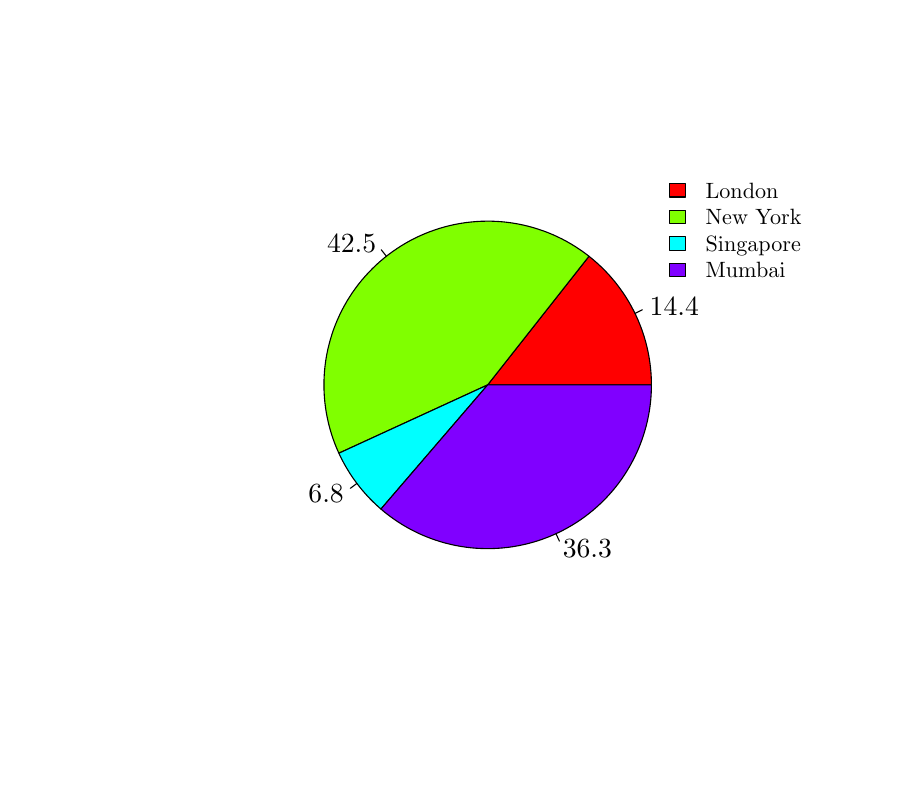
\begin{tikzpicture}[x=1pt,y=1pt]
\definecolor{fillColor}{RGB}{255,255,255}
\path[use as bounding box,fill=fillColor,fill opacity=0.00] (0,0) rectangle (308.44,270.16);
\begin{scope}
\path[clip] ( 49.20, 61.20) rectangle (283.24,220.96);
\definecolor{drawColor}{RGB}{0,0,0}
\definecolor{fillColor}{RGB}{255,0,0}

\path[draw=drawColor,line width= 0.4pt,line join=round,line cap=round,fill=fillColor] (225.39,141.08) --
	(225.36,143.06) --
	(225.26,145.04) --
	(225.09,147.01) --
	(224.86,148.98) --
	(224.56,150.93) --
	(224.20,152.88) --
	(223.77,154.81) --
	(223.28,156.73) --
	(222.73,158.63) --
	(222.11,160.52) --
	(221.42,162.37) --
	(220.68,164.21) --
	(219.88,166.02) --
	(219.01,167.80) --
	(218.09,169.55) --
	(217.11,171.27) --
	(216.07,172.96) --
	(214.97,174.61) --
	(213.82,176.22) --
	(212.62,177.80) --
	(211.36,179.33) --
	(210.06,180.82) --
	(208.70,182.26) --
	(207.30,183.66) --
	(205.85,185.01) --
	(204.36,186.31) --
	(202.83,187.56) --
	(166.22,141.08) --
	cycle;

\path[draw=drawColor,line width= 0.4pt,line join=round,line cap=round] (219.45,166.91) --
	(222.11,168.21);
\end{scope}
\begin{scope}
\path[clip] (  0.00,  0.00) rectangle (308.44,270.16);
\definecolor{drawColor}{RGB}{0,0,0}

\node[text=drawColor,anchor=base west,inner sep=0pt, outer sep=0pt, scale=  1.00] at (224.77,166.29) {14.4};
\end{scope}
\begin{scope}
\path[clip] ( 49.20, 61.20) rectangle (283.24,220.96);
\definecolor{drawColor}{RGB}{0,0,0}
\definecolor{fillColor}{RGB}{128,255,0}

\path[draw=drawColor,line width= 0.4pt,line join=round,line cap=round,fill=fillColor] (202.83,187.56) --
	(201.31,188.72) --
	(199.76,189.82) --
	(198.18,190.87) --
	(196.56,191.87) --
	(194.92,192.82) --
	(193.24,193.72) --
	(191.53,194.56) --
	(189.80,195.35) --
	(188.04,196.08) --
	(186.26,196.75) --
	(184.46,197.36) --
	(182.65,197.92) --
	(180.81,198.42) --
	(178.96,198.86) --
	(177.10,199.24) --
	(175.22,199.56) --
	(173.34,199.82) --
	(171.45,200.02) --
	(169.55,200.15) --
	(167.65,200.23) --
	(165.75,200.24) --
	(163.84,200.20) --
	(161.95,200.09) --
	(160.05,199.92) --
	(158.16,199.70) --
	(156.28,199.41) --
	(154.41,199.06) --
	(152.56,198.65) --
	(150.71,198.18) --
	(148.88,197.65) --
	(147.08,197.06) --
	(145.29,196.42) --
	(143.52,195.72) --
	(141.77,194.96) --
	(140.05,194.15) --
	(138.36,193.28) --
	(136.70,192.36) --
	(135.07,191.38) --
	(133.47,190.35) --
	(131.90,189.27) --
	(130.37,188.15) --
	(128.87,186.97) --
	(127.42,185.75) --
	(126.00,184.48) --
	(124.63,183.16) --
	(123.30,181.80) --
	(122.01,180.40) --
	(120.77,178.96) --
	(119.57,177.48) --
	(118.43,175.96) --
	(117.33,174.41) --
	(116.29,172.82) --
	(115.29,171.20) --
	(114.35,169.54) --
	(113.46,167.86) --
	(112.63,166.15) --
	(111.85,164.42) --
	(111.13,162.66) --
	(110.46,160.88) --
	(109.86,159.07) --
	(109.31,157.25) --
	(108.82,155.41) --
	(108.38,153.56) --
	(108.01,151.70) --
	(107.70,149.82) --
	(107.45,147.93) --
	(107.26,146.04) --
	(107.13,144.14) --
	(107.06,142.24) --
	(107.06,140.34) --
	(107.11,138.44) --
	(107.23,136.54) --
	(107.40,134.65) --
	(107.64,132.76) --
	(107.94,130.88) --
	(108.30,129.01) --
	(108.71,127.16) --
	(109.19,125.32) --
	(109.73,123.49) --
	(110.32,121.69) --
	(110.97,119.90) --
	(111.68,118.13) --
	(112.45,116.39) --
	(166.22,141.08) --
	cycle;

\path[draw=drawColor,line width= 0.4pt,line join=round,line cap=round] (129.62,187.56) --
	(127.78,189.89);
\end{scope}
\begin{scope}
\path[clip] (  0.00,  0.00) rectangle (308.44,270.16);
\definecolor{drawColor}{RGB}{0,0,0}

\node[text=drawColor,anchor=base east,inner sep=0pt, outer sep=0pt, scale=  1.00] at (125.95,189.01) {42.5};
\end{scope}
\begin{scope}
\path[clip] ( 49.20, 61.20) rectangle (283.24,220.96);
\definecolor{drawColor}{RGB}{0,0,0}
\definecolor{fillColor}{RGB}{0,255,255}

\path[draw=drawColor,line width= 0.4pt,line join=round,line cap=round,fill=fillColor] (112.45,116.39) --
	(113.37,114.48) --
	(114.35,112.60) --
	(115.41,110.76) --
	(116.53,108.96) --
	(117.71,107.20) --
	(118.96,105.48) --
	(120.26,103.81) --
	(121.63,102.19) --
	(123.05,100.61) --
	(124.53, 99.09) --
	(126.07, 97.62) --
	(127.65, 96.21) --
	(166.22,141.08) --
	cycle;

\path[draw=drawColor,line width= 0.4pt,line join=round,line cap=round] (118.96,105.48) --
	(116.60,103.70);
\end{scope}
\begin{scope}
\path[clip] (  0.00,  0.00) rectangle (308.44,270.16);
\definecolor{drawColor}{RGB}{0,0,0}

\node[text=drawColor,anchor=base east,inner sep=0pt, outer sep=0pt, scale=  1.00] at (114.23, 98.71) {6.8};
\end{scope}
\begin{scope}
\path[clip] ( 49.20, 61.20) rectangle (283.24,220.96);
\definecolor{drawColor}{RGB}{0,0,0}
\definecolor{fillColor}{RGB}{128,0,255}

\path[draw=drawColor,line width= 0.4pt,line join=round,line cap=round,fill=fillColor] (127.65, 96.21) --
	(129.11, 94.99) --
	(130.61, 93.83) --
	(132.15, 92.71) --
	(133.72, 91.64) --
	(135.32, 90.62) --
	(136.96, 89.65) --
	(138.63, 88.74) --
	(140.32, 87.88) --
	(142.04, 87.07) --
	(143.79, 86.33) --
	(145.56, 85.63) --
	(147.35, 85.00) --
	(149.16, 84.42) --
	(150.99, 83.90) --
	(152.84, 83.44) --
	(154.69, 83.04) --
	(156.56, 82.70) --
	(158.44, 82.42) --
	(160.33, 82.20) --
	(162.23, 82.04) --
	(164.12, 81.95) --
	(166.02, 81.91) --
	(167.92, 81.93) --
	(169.82, 82.02) --
	(171.72, 82.17) --
	(173.61, 82.37) --
	(175.49, 82.64) --
	(177.36, 82.97) --
	(179.22, 83.36) --
	(181.07, 83.80) --
	(182.90, 84.31) --
	(184.72, 84.87) --
	(186.51, 85.50) --
	(188.29, 86.18) --
	(190.04, 86.91) --
	(191.77, 87.71) --
	(193.47, 88.56) --
	(195.14, 89.46) --
	(196.78, 90.41) --
	(198.40, 91.42) --
	(199.97, 92.48) --
	(201.52, 93.59) --
	(203.02, 94.75) --
	(204.49, 95.95) --
	(205.92, 97.21) --
	(207.31, 98.50) --
	(208.66, 99.85) --
	(209.96,101.23) --
	(211.22,102.66) --
	(212.43,104.12) --
	(213.59,105.62) --
	(214.71,107.16) --
	(215.77,108.74) --
	(216.78,110.35) --
	(217.74,111.99) --
	(218.65,113.66) --
	(219.51,115.35) --
	(220.30,117.08) --
	(221.05,118.83) --
	(221.73,120.60) --
	(222.36,122.40) --
	(222.93,124.21) --
	(223.45,126.04) --
	(223.90,127.88) --
	(224.29,129.74) --
	(224.63,131.61) --
	(224.90,133.50) --
	(225.12,135.38) --
	(225.27,137.28) --
	(225.36,139.18) --
	(225.39,141.08) --
	(166.22,141.08) --
	cycle;

\path[draw=drawColor,line width= 0.4pt,line join=round,line cap=round] (190.91, 87.30) --
	(192.14, 84.62);
\end{scope}
\begin{scope}
\path[clip] (  0.00,  0.00) rectangle (308.44,270.16);
\definecolor{drawColor}{RGB}{0,0,0}

\node[text=drawColor,anchor=base west,inner sep=0pt, outer sep=0pt, scale=  1.00] at (193.37, 78.72) {36.3};
\end{scope}
\begin{scope}
\path[clip] ( 49.20, 61.20) rectangle (283.24,220.96);
\definecolor{drawColor}{RGB}{0,0,0}
\definecolor{fillColor}{RGB}{255,0,0}

\path[draw=drawColor,line width= 0.4pt,line join=round,line cap=round,fill=fillColor] (232.00,213.76) rectangle (237.76,208.96);
\definecolor{fillColor}{RGB}{128,255,0}

\path[draw=drawColor,line width= 0.4pt,line join=round,line cap=round,fill=fillColor] (232.00,204.16) rectangle (237.76,199.36);
\definecolor{fillColor}{RGB}{0,255,255}

\path[draw=drawColor,line width= 0.4pt,line join=round,line cap=round,fill=fillColor] (232.00,194.56) rectangle (237.76,189.76);
\definecolor{fillColor}{RGB}{128,0,255}

\path[draw=drawColor,line width= 0.4pt,line join=round,line cap=round,fill=fillColor] (232.00,184.96) rectangle (237.76,180.16);

\node[text=drawColor,anchor=base west,inner sep=0pt, outer sep=0pt, scale=  0.80] at (244.96,208.60) {London};

\node[text=drawColor,anchor=base west,inner sep=0pt, outer sep=0pt, scale=  0.80] at (244.96,199.00) {New York};

\node[text=drawColor,anchor=base west,inner sep=0pt, outer sep=0pt, scale=  0.80] at (244.96,189.40) {Singapore};

\node[text=drawColor,anchor=base west,inner sep=0pt, outer sep=0pt, scale=  0.80] at (244.96,179.80) {Mumbai};
\end{scope}
\end{tikzpicture}

    \caption{Diagrama de \textit{pizza}.}
    \label{graph:pie-plot}
\end{figure}


